\begin{figure}[htb]
  \begin{center}
    \resizebox{0.9\linewidth}{!}{
      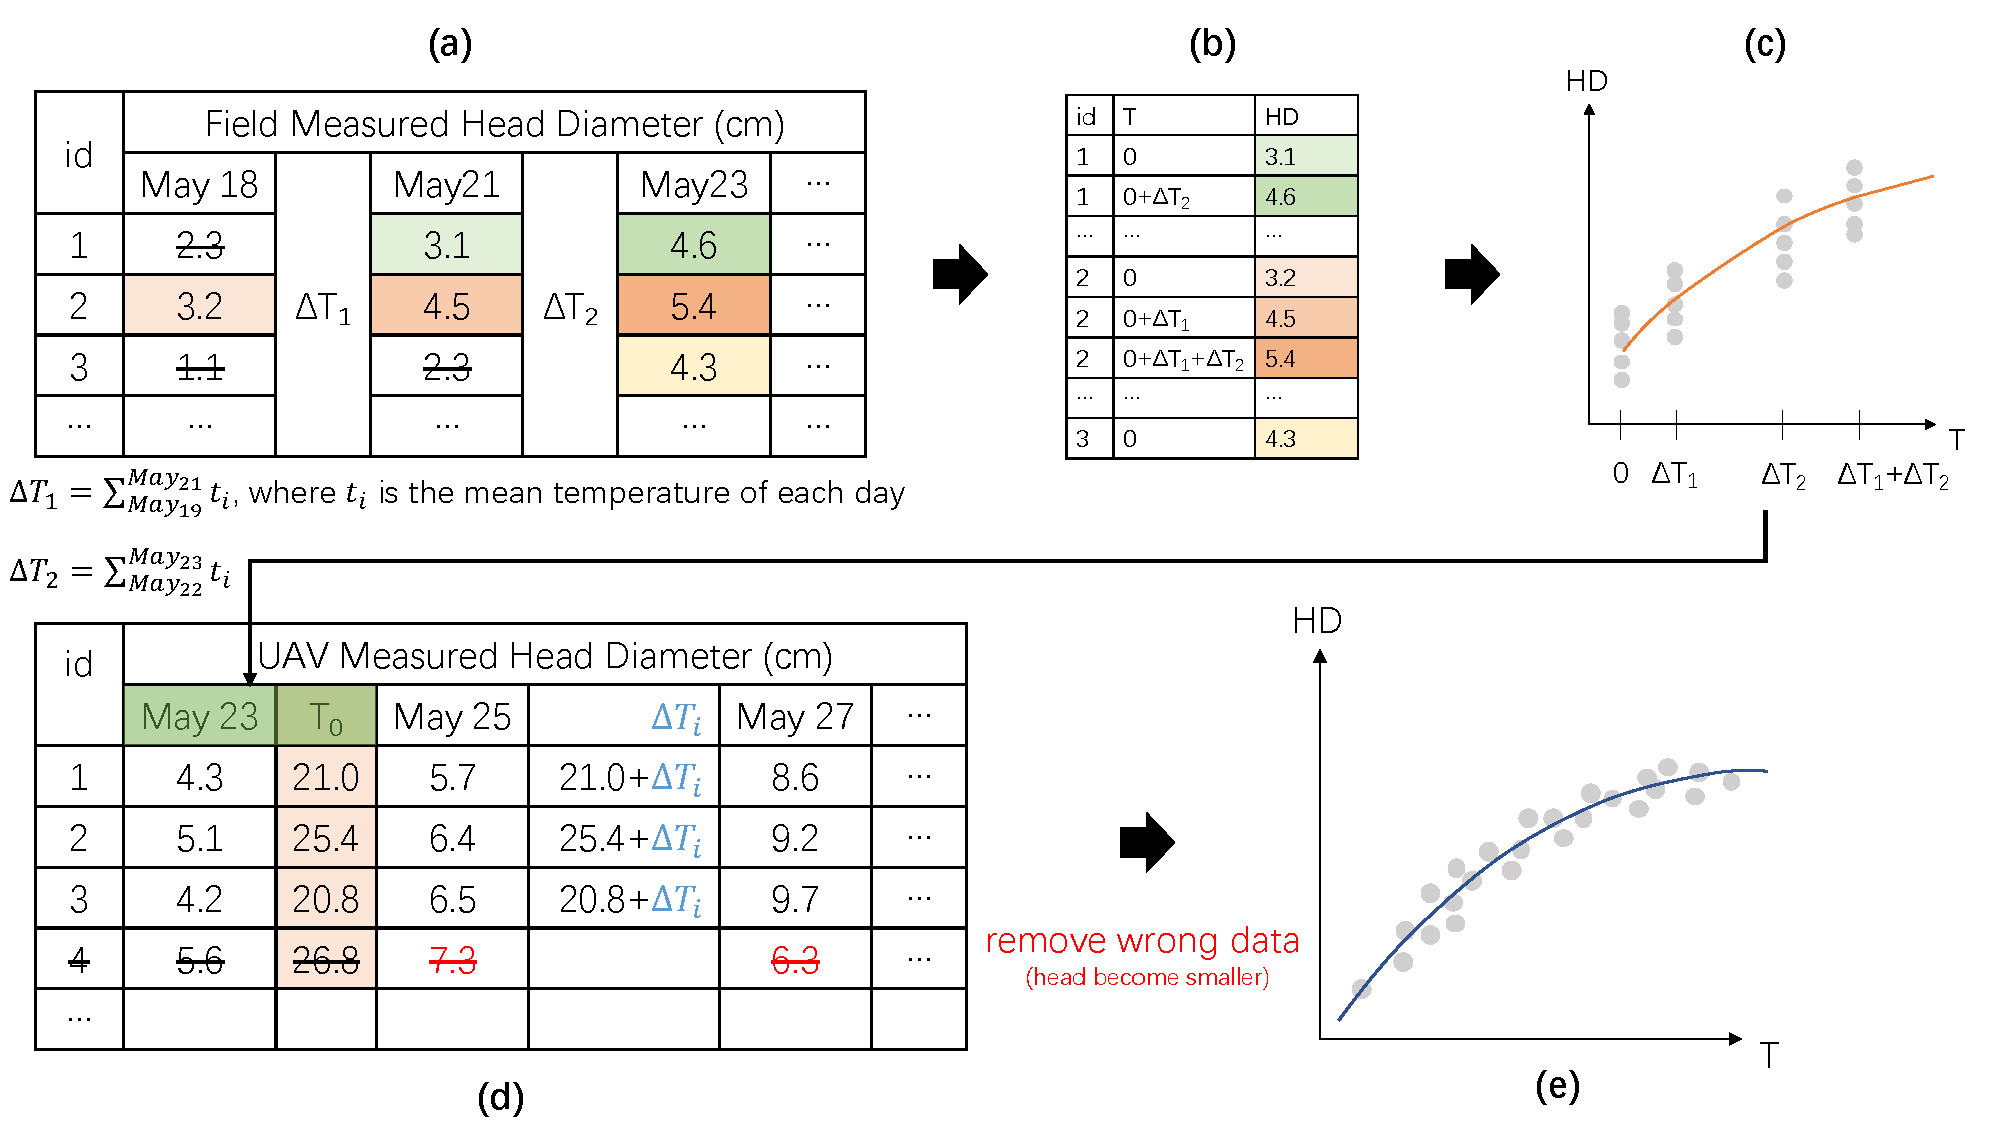
\includegraphics{figures/bro/Fig.S3_yield_workflow.pdf}
    }
  \end{center}
  \caption[Data processing illustration for head size prediction model]{
    Data processing illustration for head size prediction model. All the numbers were just examples, not the actual results. 
    (a) The field-measured measured diameter at on different dates; the light colored was used as the starting date with broccoli head size around of approximately 3-3.5cm. $T$ is the sum of daily average temperature. $\Delta T_i$ is the temperature sum deviation. 
    (b) Reshaping of the previous table to a two-column table for the regression analysis shown in (c). 
    (d) The previous regressed model was used to initialize the $T$ from the head diameter. 
    $T$ on later days was added by the deviation $\Delta T_i$. 
    (e) the previous data was used to regress the prediction model from $T$ to head diameter.
  }
  \label{fig:bros3}
\end{figure}